%%
%% Copyright 2007, 2008, 2009 Elsevier Ltd
%%
%% This file is part of the 'Elsarticle Bundle'.
%% ---------------------------------------------
%%
%% It may be distributed under the conditions of the LaTeX Project Public
%% License, either version 1.2 of this license or (at your option) any
%% later version.  The latest version of this license is in
%%    http://www.latex-project.org/lppl.txt
%% and version 1.2 or later is part of all distributions of LaTeX
%% version 1999/12/01 or later.
%%
%% The list of all files belonging to the 'Elsarticle Bundle' is
%% given in the file `manifest.txt'.
%%

%% Template article for Elsevier's document class `elsarticle'
%% with numbered style bibliographic references
%% SP 2008/03/01
%%
%%
%%
%% $Id: elsarticle-template-num.tex 4 2009-10-24 08:22:58Z rishi $
%%
%%
\documentclass[preprint,12pt]{elsarticle}

%% Use the option review to obtain double line spacing
%% \documentclass[preprint,review,12pt]{elsarticle}

%% Use the options 1p,twocolumn; 3p; 3p,twocolumn; 5p; or 5p,twocolumn
%% for a journal layout:
%\documentclass[final,1p,times]{elsarticle}
%\documentclass[final,1p,times,twocolumn]{elsarticle}
%% \documentclass[final,3p,times]{elsarticle}
%% \documentclass[final,3p,times,twocolumn]{elsarticle}
%% \documentclass[final,5p,times]{elsarticle}
%% \documentclass[final,5p,times,twocolumn]{elsarticle}

%% if you use PostScript figures in your article
%% use the graphics package for simple commands
%% \usepackage{graphics}
%% or use the graphicx package for more complicated commands
 \usepackage{graphicx}
%% or use the epsfig package if you prefer to use the old commands
%% \usepackage{epsfig}
\usepackage{graphics}
%% The amssymb package provides various useful mathematical symbols
\usepackage{amssymb}
%% The amsthm package provides extended theorem environments
 \usepackage{amsthm}
\usepackage{amsfonts}
\usepackage{amsmath}
\usepackage{booktabs}
\usepackage{bm}
\def\MLine#1{\par\hspace*{-\leftmargin}\parbox{\textwidth}{\[#1\]}}

\newcommand{\obj}[1] {\textit{#1}}
\newcommand{\sr}[1] {\textbf{#1}}
\newcommand{\rcc}[1] {\texttt{#1}}
\newcommand{\class}[1] {\textsf{#1}}


\newcommand{\const}[1] {$\mathit{#1}$}
\newcommand{\constsmall}[1] {\small $\mathit{#1}$}
\newcommand{\objvar}[1] {$\mathsf{#1}$}
\newcommand{\stvar}[1] {\textsf{#1}}
\newcommand{\stvarsmall}[1] {\small {\textsf{#1}}}
\newcommand{\op}[1] {\textsl{#1}}

%% The lineno packages adds line numbers. Start line numbering with
%% \begin{linenumbers}, end it with \end{linenumbers}. Or switch it on
%% for the whole article with \linenumbers after \end{frontmatter}.
% \usepackage{lineno}

%% natbib.sty is loaded by default. However, natbib options can be
%% provided with \biboptions{...} command. Following options are
%% valid:

%%   round  -  round parentheses are used (default)
%%   square -  square brackets are used   [option]
%%   curly  -  curly braces are used      {option}
%%   angle  -  angle brackets are used    <option>
%%   semicolon  -  multiple citations separated by semi-colon
%%   colon  - same as semicolon, an earlier confusion
%%   comma  -  separated by comma
%%   numbers-  selects numerical citations
%%   super  -  numerical citations as superscripts
%%   sort   -  sorts multiple citations according to order in ref. list
%%   sort&compress   -  like sort, but also compresses numerical citations
%%   compress - compresses without sorting
%%
%% \biboptions{comma,round}

% \biboptions{}


\journal{Robotics and Automation Systems}

\begin{document}

\begin{frontmatter}

%% Title, authors and addresses

%% use the tnoteref command within \title for footnotes;
%% use the tnotetext command for the associated footnote;
%% use the fnref command within \author or \address for footnotes;
%% use the fntext command for the associated footnote;
%% use the corref command within \author for corresponding author footnotes;
%% use the cortext command for the associated footnote;
%% use the ead command for the email address,
%% and the form \ead[url] for the home page:
%%
% \title{Title\tnoteref{label1}}
% \tnotetext[label1]{}
% \author{Name\corref{cor1}\fnref{label2}}
% \ead{email address}
% \ead[url]{home page}
% \fntext[label2]{}
% \cortext[cor1]{}
% \address{Address\fnref{label3}}
% \fntext[label3]{}

\title{SIRO: State-Based Intention Recognition Using Ontologies in Cooperative Human-Robot Environments}

%% use optional labels to link authors explicitly to addresses:
 \author[nist,le2i]{Craig Schlenoff\corref{cor1}}
 \ead{craig.schlenoff@nist.gov}

 \author[nist]{Anthony Pietromartire}
 \ead{pietromartire.anthony@nist.gov}

 \author[umd]{Zeid Kootbally}
 \ead{zeid.kootbally@nist.gov}

 \author[nist]{Stephen Balakirsky}
 \ead{stephen.balakirsky@nist.gov}

 \author[qatar,le2i]{Sebti Foufou}
 \ead{sfoufou@qu.edu.qa}

 \address[nist]{National Institute of Standards and Technology (NIST), 100 Bureau Drive, Stop 8230, Gaithersburg MD 20899 USA}
 \address[le2i]{University of Burgundy, LE2i Lab, Dijon, France}
 \address[qatar]{Computer Science and Engineering Department Qatar University, Doha Qatar}
 \address[umd]{University of Maryland, Department of Mechanical Engineering, College Park MD 20742 USA}
 \cortext[cor1]{Corresponding author: 301-975-3456}

%\author{}
%\address{}

\begin{abstract}
In this paper, we describe a novel approach for representing state information for the purpose of intention recognition in cooperative human-robot environments. States are represented by a combination of spatial relationships in a Cartesian frame along with cardinal direction information. This approach is applied to a manufacturing kitting operation, where humans and robots are working together to develop kits. Based upon a set of predefined high-level states relationships that must be true for future actions to occur, a robot can use the detailed state information described in this paper to infer the probability of subsequent actions occurring. This would allow the robot to better help the human with the task or, at a minimum, better stay out of his or her way.
\end{abstract}

\begin{keyword}
Intention recognition \sep state-based representation \sep ontologies \sep human robot safety \sep RCC8

\end{keyword}

\end{frontmatter}

%%
%% Start line numbering here if you want
%%
% \linenumbers

%% main text
\section{Introduction}
\label{S:INTRO}

Humans and robots working safely and seamlessly together in a cooperative environment is one of the future goals of the robotics community. When humans and robots can work together in the same space, a whole class of tasks becomes amenable to automation, ranging from collaborative assembly, to parts and material handling and delivery. Keeping humans safe requires the ability of the robot to monitor the work area, infer human intention, and be aware of potential dangers soon enough to avoid them. Robots are under development throughout the world that will revolutionize manufacturing by allowing humans and robots to operate in close proximity while performing a variety of tasks~\cite{SZABO.2011}.

Proposed standards exist for robot-human safety, but these standards focus on robots adjusting their speed based on the separation distance between the human and the robot~\cite{CHABROL.1987}. In essence, as the robot gets closer to a detected human, the robot gradually decreases its speed to ensure that if a collision between the human and robot occurs, minimal damage will be caused. The approaches focus on where the human is at a given point in time. It does not focus on where they are anticipated to be at points in the future.

A key enabler for human-robot safety in cooperative environments involves the field of intention recognition, in which the robot attempts to understand the intention of an agent (the human) by recognizing some or all of their actions~\cite{SADRI.2011} to help predict the human's future actions. Knowing these future actions will allow a robot to plan in such a way as to either help the human perform his/her activities or, at a minimum, not put itself in a position to cause an unsafe situation.

In this paper, we present an approach to representing state information in an ontology for the purpose of ontology-based intention recognition. This is an extension to the conference paper~\cite{SCHLENOFF.UBICOMP.2012} presented at the Ubiquitous Computing Conference, Workshop on Ubiquitous Robotics. In this context, a state is defined as a set of properties of one or more objects in an area of interest that consist of specific recognizable configuration(s) and or characteristic(s). A state is composed of one to many state relationships, which is a specific relation between two objects (e.g., Object 1 is on top of Object 2). This approach to intention recognition is different than many ontology-based intention recognition approaches in the literature (as described in the section 2) as they primarily focus on activity (as opposed to state) recognition and then use a form of abduction to provide explanations for observations. We infer detailed state relationships using observations based on Region Connection Calculus 8 (RCC8)~\cite{RANDELL.ICKRR.1992} and other cardinal relationships and then combine these observations to infer the overall state relationships that are true at a given time. The advantages of using state representation over activity representation to perform intention recognition is documented in~\cite{SCHLENOFF.ECDRM.2012}. The core concept is that states tend to be easier to recognize than activities, thus allowing for more accurate input into intention recognition systems. Once a sequence of state relationships has been identified, we use probabilistic procedures to associate those states with likely overall intentions to determine the next possible action (and associated state) that is likely to occur. This paper focuses on the way that states are represented, reasoned over, and updated in the ontology. The way that the states are combined to represent intentions is only lightly described in this paper. The reader is referred to~\cite{SCHLENOFF.ECDRM.2012} for more information about this topic. The value that this journal article provides is a general approach for the recognition and representation of states in the environment for the purpose of intention recognition as well as the application of this approach to the manufacturing kitting domain.

We start by providing an overview of intention recognition efforts in the literature as well as various approaches for ontology-based state representation. The approach to state recognition is then presented. Because the ontology is meant to be a more permanent form of knowledge representation and does not need to be updated with every new state detected, we explain the logic employed to determine when the ontology should be updated. We then present a manufacturing kitting scenario along with a corresponding kitting ontology and we apply the state representation approach to this domain. Lastly, we describe the results of an implementation of these state-based approaches in a simulation environment.
%%%%%%%%%%%%%%%%%%%%%%%%%%%%%%%%%%%%%%%%%%%%%%%%%%%%%%%%%%%%%%%%%%%%%%%%%%%%%%%%%%%%%%%%%
\section{Intention Recognition and State Representation Related Work }\label{S:section1}
%%%%%%%%%%%%%%%%%%%%%%%%%%%%%%%%%%%%%%%%%%%%%%%%%%%%%%%%%%%%%%%%%%%%%%%%%%%%%%%%%%%%%%%%%
Intention recognition traditionally involves recognizing the intent of an agent by analyzing some of, or all of, the actions that the agent performs. Many of the recognition efforts in the literature are composed of at least three components: (1) identification and representation of a set of intentions that are relevant to the domain of interest, (2) representation of a set of actions that are expected to be performed in the domain of interest and the association of these actions with the intentions, (3) recognition of a sequence of observed actions executed by the agent and matching them to the actions in the representation~\cite{SADRI.2011}.


There have been many techniques in the literature applied to intention recognition that follow the three steps listed above, including an ontology-based approach~\cite{JEON.ICMUE.2008}, multiple probabilistic frameworks such as  Hidden Markov Models~\cite{KELLEY.ICHRI.2008} and Dynamic Bayesian Networks~\cite{SCHREMPF.ICAR.2005}, utility-based intention recognition~\cite{MAO.AAMAS.2004}, and graph-based intention recognition~\cite{YOUN.IJASET.2008}. In this paper, we focus on ontology/logic-based approaches.


Once observations of actions have been made, different approaches exist to match those observations to an overall intention or goal. For example, in~\cite{MULDER.IF.2003}, the authors use existentially quantified observations (not fully grounded observations) to match actions to plan libraries. Mulder can handle situations when they see an action occur (e.g., opening a door), without seeing or knowing who performed that action Other approaches have focused on building plans with frequency information, to represent how often an activity occurs~\cite{JARVIS.AIM.2005}. The rationale behind these approaches is that there are some activities that occur very frequently and are often not relevant to the recognition process (e.g., a person cleaning his/her hands). These frequently-occurring activities can be mostly ignored, and only activities that are less commonly performed can be considered. In~\cite{DEMOLOMBE.CLIMA.2005}, the authors combine probabilities and situation calculus-like formalization of actions. In particular, Demolombe not only define the actions and sequences of actions that constitute an intention, they also state which activities cannot occur for the intention to be valid. For example, if the intention was to drive a car, the activity may be to open the door, get into the car, turn on the engine, release the emergency brake, and take the car out of park. Demolombe may also include that an activity cannot be to turn the car off after it is turned on and before the car is taken out of park.

All of these approaches have focused on the activity being performed as the primary basis for observation and the building block for intention recognition. However, as noted in~\cite{SADRI.2011}, activity recognition is a very hard problem and one that is far from being solved. There has been limited success in using Radio Frequency Identification (RFID) readers and tags attached to objects of interest to track their movement with the goal of associating their movement with known activities. For example, in~\cite{Philipose.PC.2004}, the authors describe the process of making tea as a three step process involving using a kettle, getting a box of tea bags, and adding some combination of milk, sugar or lemon. Each of these activities is identified by a user wearing a special set of gloves that can read RFID tags on objects of interest. However, this additional hardware can be inhibiting and unnatural.  Recognizing and representing states as opposed to actions can help to address some of the issues involved in activity recognition (e.g., the location of the tea bag box and the milk carton with respect to the tea cup) will be the focus of the rest of this paper.


State representation is documented in the literature, although it has not been used (to the authors knowledge) for ontology-based intention recognition. An important aspect of an object's state is its spatial relationships to other objects. In~\cite{Bateman.2006}, an overview is given that describes the way that spatial information is represented in various upper ontologies including the Descriptive Ontology for Linguistics and Cognitive Engineering (DOLCE), Cyc, the Standard Upper Merged Ontology (SUMO), and Basic Formal Ontology (BFO). The conclusion of this work is the identification of a list of high-level requirements that were necessary for any spatial ontology, including:

\begin{itemize}
\item A selection of an appropriate granular partition of the world that picks out the entity that we wish to locate with respect to other entities.
\item A selection of an appropriate space region formalization that brings out or makes available relevant spatial relationships.
\item A selection of an appropriate partition over the space region (e.g., RCC8, qualitative distance, cardinal direction).
\item The identification of the location of the entity with respect to the selected space region description.
\end{itemize}
Bateman ended up using a variation of the DOLCE ontology, but there is no mention in the literature about the detailed spatial relations that were developed as part of this effort.


Region Connected Calculus (RCC8)~\cite{Wolter.KR.2000} is a well-known and cited approach for representing the relationship between two regions in Euclidean space or in a topological space. There are eight possible relations, including disconnected, externally connected, partially overlapping, etc. However, RCC8 only addresses these relationships in two-dimensional space. There have been other approaches that have tried to extend this into a region connected calculus in three-dimensional space while addressing occlusions~\cite{Albath.CAINE.2010}. There have also been other approaches to develop calculi for spatial relations. FlipFlop calculus~\cite{Ligozat.1993} describes the position of one point (the referent) in a plane with respect to two other points (the origin and the relatum). Single Cross Calculus (SCC)~\cite{Freksa.LNCS.1992}  is a ternary calculus that describes the direction of a point (C - the referent) with respect to a second point (B - the relatum) as seen from a third point (A - the origin) in a plane. Double Cross Calculus (DCC)~\cite{Freksa.LNCS.1992} extends SCC by allowing one to also determine the relative location of point A with respect to point B (in addition to point B with respect to point A as in SCC). Coarse-grained Dipole Relation Algebra~\cite{Schlieder.1995} describes the orientation relation between two dipoles (an oriented line segment as determined by a start and end point). Oriented Point Relation Algebra (OPRA)~\cite{Moratz.IJCAI.2005} relates two oriented points (a point in a plane with an additional direction parameter) and describes their relative orientation towards each other. All of these approaches, apart from RCC8, focus on points and lines as opposed to regions. Also, despite the large variety of qualitative spatial calculi, the amount of applications employing qualitative spatial reasoning techniques is comparatively small~\cite{Wallgrun.ICSC.2007}.

Throughout the rest of this paper, we will describe an approach for ontology-based state representation within the context of a typical manufacturing scenario.

%%%%%%%%%%%%%%%%%%%%%%%%%%%%%%%%%%%%%%%%%%%%%%%%%%%%%%%%%%%%%%%%%%%%%%%%%%%%%%%%%%%%%
\section{Representing States and Spatial Relations in the Ontology}\label{S:section2}
%%%%%%%%%%%%%%%%%%%%%%%%%%%%%%%%%%%%%%%%%%%%%%%%%%%%%%%%%%%%%%%%%%%%%%%%%%%%%%%%%%%%%
In this section, we describe an approach that uses RCC8 to model state relationships based on the relative position of objects in the environment. However, we will extend RCC8, which was initially developed for a two-dimensional space, to a three-dimensions space by applying it along all three planes (x-y, x-z, y-z). The frame of reference will be with respect to the fixed object (e.g., a worktable), with the z-dimension pointing straight upwards and the tabletop extending in the x- and y- dimension (with detailed orientation specific to the application).  Each of the high-level state relationships (to be discusses later in the paper) will have a set of logical rules that associate these RCC8 relations to them. These RCC8 relations should easily allow a sensor system to characterize the corresponding state relations.

\subsection{RCC8 Approach}
As mentioned earlier, RCC8 abstractly describes regions in Euclidean or topological space by their relations to each other. RCC8 consists of eight basic relations that are possible between any two regions:

\begin{itemize}
  \item Disconnected (DC)
  \item Externally Connected (EC)
  \item Equal (EQ)
  \item Partially Overlapping (PO)
  \item Tangential Proper Part (TPP)
  \item Non-Tangential Proper Part (NTPP)
  \item Tangential Proper Part Inverse (TPPi)
  \item Non-Tangential Proper Part Inverse (NTPPi)
\end{itemize}

These are shown pictorially in Figure~\ref{fig:RCC8}.
%%%%%%%%%%%%%%%%%%%%%%%%%%%% --> Fig

\begin{figure}[h!t!]
\begin{center}
\begin{tabular}{c}
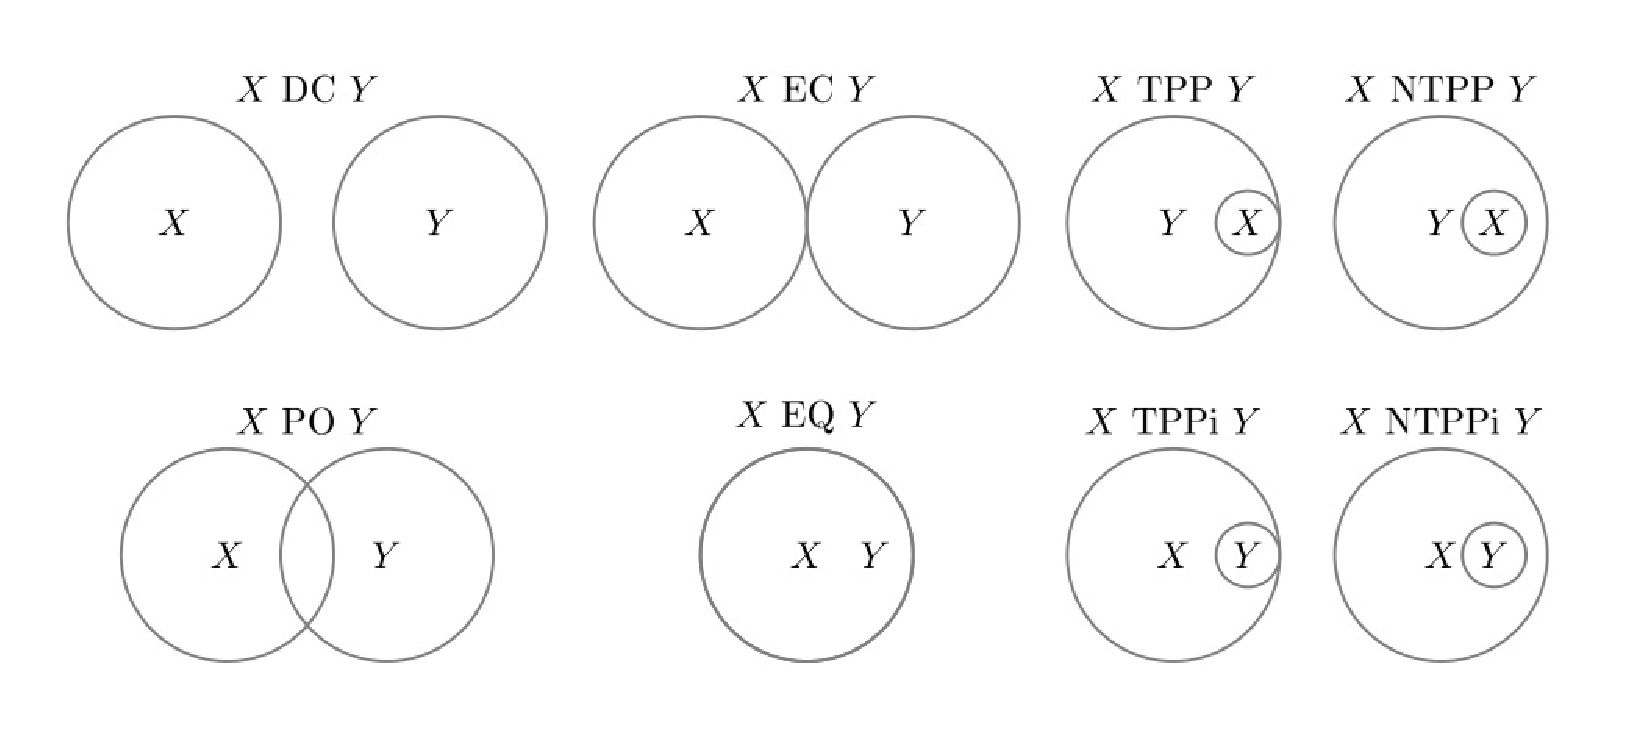
\includegraphics[width=12cm]{rcc8.eps}
\end{tabular}
\end{center}
\caption{RCC8 Relations (credit: http://en.wikipedia.org/wiki/RCC8).}
\label{fig:RCC8}
\end{figure}

RCC8 was created to model the relationships between two regions in two dimensions. In many domains, these relations need to be modeled in all three dimensions. As such, every pair of objects has a RCC8 relation in all three dimensions. To address this, we are prepending an x-, y- or z- before each of the RCC8 relations. For example, to represent the RCC8 relations in the x-dimension, the nomenclature would be:
\begin{itemize}
  \item \rcc{x-DC}
  \item \rcc{x-EC}
  \item \rcc{x-EQ}
  \item \rcc{x-PO}
  \item \rcc{x-TPP}
  \item \rcc{x-NTPP}
  \item \rcc{x-TPPi}
  \item \rcc{x-NTPPi}
\end{itemize}

Similar nomenclature would be used in the y- and z- dimensions. The combination of all 24 RCC relations starts to describe the spatial relations between any two objects in the scene. However, more information is needed to represent the cardinal direction between any two objects. For example, to state that a worktable is empty (worktable-empty(worktable)), one needs to state that there is nothing on top of it. If we assume that the vertical dimension is the z-dimension, then saying that:

\begin{equation}\label{eq:z-EC}
\texttt{z-EC}(\textit{worktable}, \textit{obj1})
\end{equation}
%\begin{center}\texttt{z-EC}(\textit{worktable}, \textit{obj1})\end{center}

(which intuitively means \obj{obj1} is externally connected to the \obj{worktable} in the z-dimension) is not sufficient because \obj{obj1} could be either on top of or below the \obj{worktable}. In other words, we need to represent directionality. We do this using the following Boolean operators:

\begin{equation}\label{eq:greater-x}
\texttt{greater-x}(\textit{A}, \textit{B})
\end{equation}
\begin{equation}\label{eq:smaller-x}
\texttt{smaller-x}(\textit{A}, \textit{B})
\end{equation}
\begin{equation}\label{eq:greater-y}
\texttt{greater-y}(\textit{A}, \textit{B})
\end{equation}
\begin{equation}\label{eq:smaller-y}
\texttt{smaller-y}(\textit{A}, \textit{B})
\end{equation}
\begin{equation}\label{eq:greater-z}
\texttt{greater-z}(\textit{A}, \textit{B})
\end{equation}
\begin{equation}\label{eq:smaller-z}
\texttt{smaller-z}(\textit{A}, \textit{B})
\end{equation}

which intuitively means, in Equation~\ref{eq:greater-x}, that the edge of the bounding plane of object \textit{A} is greater than (in the x-dimension in the defined frame of reference) the edge of the bounding plane of object \textit{B}.

\subsection{Defining More Complex Relations}
There are undoubtedly many other relationships that may be needed in the future to describe a scene of interest. These could include absolute locations and orientations of objects (x, y, z, roll, pitch, yaw) and relative distance (closer, farther, etc.). However, these spatial relations are sufficient for describing the manufacturing kitting example later in this paper.

From these RCC8 spatial relations, we can define more complex spatial relations such as the ones below:
\begin{itemize}
  \item \sr{Contained-In} - an object is enclosed in a second object from all sides
  \item \sr{Not-Contained-In} - an object is not enclosed in a second object from all sides
  \item \sr{Partially-In} - an object is inside of another object in at least two dimensions but not fully contained in
  \item \sr{In-Contact-With} - touching at least one side and not contained with (i.e., touching outer edges)
  \item \sr{On-Top-Of} - the edge of the bounding plane of one object is greater (in the z-dimension) than that of a second object
  \item \sr{Under} - the edge of the bounding plane of one object is less (in the z-dimension) than a second object
\end{itemize}

And from these, we can define composite spatial relationships such as:
\begin{itemize}
  \item \sr{Under-And-In-Contact-With} - an object is both under and in contact with a second object
  \item \sr{Partially-In-And-In-Contact-With} - an object is inside of another object in at least two dimensions and touching the object in at least one dimension
\end{itemize}
Below,we formalize these spatial relationships by defining them using the RCC8 state representation. In natural language, Equation~\ref{eq:contained-in} below states that object 1 (\obj{obj1}) is contained in object 2 (\obj{obj2}) if \obj{obj1} is tangentially or non-tangentially a proper part of \obj{obj2} in the x, y, and z-dimension. One can logically envision this by drawing two convex figures, and the first convex hull is completely inside of the second convex hull in all three dimensions, with it touching or not touching the second convex hull in all of the three dimensions.
\begin{gather}
\label{eq:contained-in}
\textbf{Contained-In}(\textit{obj1}, \textit{obj2}) \rightarrow  \\
(\texttt{x-TPP}(\textit{obj1}, \textit{obj2}) \vee \texttt{x-NTPP}(\textit{obj1}, \textit{obj2})) \wedge \notag\\
(\texttt{y-TPP}(\textit{obj1}, \textit{obj2}) \vee \texttt{y-NTPP}(\textit{obj1}, \textit{obj2})) \wedge \notag\\
(\texttt{z-TPP}(\textit{obj1}, \textit{obj2}) \vee \texttt{z-NTPP}(\textit{obj1}, \textit{obj2}))\notag
\end{gather}
\begin{gather}
\label{eq:not-contained-in}
\textbf{Not-Contained-In}(\textit{obj1}, \textit{obj2}) \rightarrow\\
\neg \textbf{Contained-In}(\textit{obj1}, \textit{obj2}) \notag
\end{gather}
\begin{gather}
\label{eq:partially-in}
\textbf{Partially-In}(\textit{obj1}, \textit{obj2}) \rightarrow \\
\textbf{Not-Contained-In}(\textit{obj1}, \textit{obj2}) \wedge \notag\\
((\texttt{x-TPP}(\textit{obj1}, \textit{obj2}) \vee \texttt{x-NTPP}(\textit{obj1}, \textit{obj2})) \wedge  \notag\\
(\texttt{y-TPP}(\textit{obj1}, \textit{obj2}) \vee \texttt{y-NTPP}(\textit{obj1}, \textit{obj2}))) \vee  \notag\\
((\texttt{x-TPP}(\textit{obj1}, \textit{obj2}) \vee \texttt{x-NTPP}(\textit{obj1}, \textit{obj2})) \wedge  \notag\\
(\texttt{z-TPP}(\textit{obj1}, \textit{obj2}) \vee \texttt{z-NTPP}(\textit{obj1}, \textit{obj2}))) \vee  \notag\\
((\texttt{y-TPP}(\textit{obj1}, \textit{obj2}) \vee \texttt{y-NTPP}(\textit{obj1}, \textit{obj2})) \wedge  \notag\\
(\texttt{z-TPP}(\textit{obj1}, \textit{obj2}) \vee \texttt{z-NTPP}(\textit{obj1}, \textit{obj2}))) \notag
\end{gather}
\begin{gather}
\label{eq:in-contact-with}
\textbf{In-Contact-With}(\textit{obj1}, \textit{obj2}) \rightarrow \\
\texttt{x-EC}(\textit{obj1}, \textit{obj2}) \vee \texttt{y-EC}(\textit{obj1}, \textit{obj2}) \vee \texttt{z-EC}(\textit{obj1}, \textit{obj2})\notag
\end{gather}
\begin{gather}
\label{eq:on-top-of}
\textbf{On-Top-Of}(\textit{obj1}, \textit{obj2}) \rightarrow \vee \\
\texttt{greater-z}(\textit{obj1}, \textit{obj2}) \wedge ((\texttt{x-EQ}(\textit{obj1}, \textit{obj2}) \vee \texttt{x-NTPP}(\textit{obj1}, \textit{obj2}) \vee \notag\\
\texttt{x-TPP}(\textit{obj1}, \textit{obj2}) \vee \texttt{x-PO}(\textit{obj1}, \textit{obj2}) \vee \texttt{x-NTPPi}(\textit{obj1}, \textit{obj2}) \vee \notag\\
\texttt{x-TPPi}(\textit{obj1}, \textit{obj2})) \wedge ((\texttt{y-EQ}(\textit{obj1}, \textit{obj2}) \vee \texttt{y-NTPP}(\textit{obj1}, \textit{obj2}) \vee \notag\\
\texttt{y-TPP}(\textit{obj1}, \textit{obj2}) \vee \texttt{y-PO}(\textit{obj1}, \textit{obj2}) \vee \texttt{y-NTPPi}(\textit{obj1}, \textit{obj2}) \vee \notag\\
\texttt{y-TPPi}(\textit{obj1}, \textit{obj2})) \notag
\end{gather}
\begin{gather}
\label{eq:under}
\textbf{Under}(\textit{obj1}, \textit{obj2}) \rightarrow \\
\texttt{smaller-z}(\textit{obj1}, \textit{obj2}) \wedge ((\texttt{x-EC}(\textit{obj1}, \textit{obj2}) \vee \texttt{x-NTPP}(\textit{obj1}, \textit{obj2}) \vee  \notag\\
\texttt{x-TPP}(\textit{obj1}, \textit{obj2}) \vee \texttt{x-PO}(\textit{obj1}, \textit{obj2}) \vee \texttt{x-NTPPi}(\textit{obj1}, \textit{obj2}) \vee  \notag\\
\texttt{x-TPPi}(\textit{obj1}, \textit{obj2})) \wedge ((\texttt{y-EC}(\textit{obj1}, \textit{obj2}) \vee \texttt{y-NTPP}(\textit{obj1}, \textit{obj2}) \vee  \notag\\
\texttt{y-TPP}(\textit{obj1}, \textit{obj2}) \vee \texttt{y-PO}(\textit{obj1}, \textit{obj2}) \vee \texttt{y-NTPPi}(\textit{obj1}, \textit{obj2}) \vee  \notag\\
\texttt{y-TPPi}(\textit{obj1}, \textit{obj2})) \notag
\end{gather}
\begin{gather}
\label{eq:Under-And-In-Contact-With}
\textbf{Under-And-In-Contact-With}(\textit{obj1}, \textit{obj2}) \rightarrow \\
\textbf{Under}(\textit{obj1}, \textit{obj2}) \wedge \textbf{In-Contact-With}(\textit{obj1}, \textit{obj2})\notag
\end{gather}

\begin{gather}
\label{eq:Partially-In-And-In-Contact-With}
\textbf{Partially-In-And-In-Contact-With}(\textit{obj1}, \textit{obj2}) \rightarrow\\
\textbf{Partially-In}(\textit{obj1}, \textit{obj2}) \wedge \textbf{In-Contact-With}(\textit{obj1}, \textit{obj2})\notag
\end{gather}

These spatial relationships will be used later in the paper to define two manufacturing kitting intentions.

\subsection{How States are Represented in the Ontology}
The spatial relations above are represented as subclasses of the \class{RelativeLocation} class which is a subtype of the \class{PhysicalLocation} class which is a subtype of \class{DataThing} class in the ontology (to be discussed in more detail later in the paper). \class{DataThings} are abstract, non-tangible things that are classes in the ontology. There are three types of spatial relations, each described below:
\begin{itemize}
\item \textbf{RCC8\_Relations} - These are the 24 RCC8 relations and the six cardinality direction operators described earlier in this section. These classes are not any further defined but can be instantiated as occurrences of them are found in the environment.
\item \textbf{Intermediate\_State\_Relations} - These are intermediate level state relations that can be inferred from the combination of RCC8 and cardinal direction relations. The examples above such as \sr{Under} and \sr{In-Contact-With} are examples of state relations. The logical expression based on the RCC8 and cardinal direction relations (as shown in Equations~\ref{eq:contained-in}--\ref{eq:Partially-In-And-In-Contact-With}) which are evaluated to determine that truth-value of the state relation are represented within the Equivalent Classes. The information is exported from the ontology during run-time and converted into code that is evaluated as new perception data is presented to the system.
\item \textbf{Predicates} - These are domain-specific states that are of interest current intention (or set of intentions) being evaluated. For example, in the manufacturing example to be discussed later in the paper, one state of interest is that the worktable is empty. This is true if the worktable is not \sr{Under-And-In-Contact-With} any object. The truth-value of predicates can be determined through the logical combination of state relations. As with state relations, this is captured using the equivalent classes in the ontology.
\end{itemize}


\subsection{Reading and Writing From the Ontology}
The purpose of representing state information is to try to determine the intention that is being performed by a human in the environment. It is impractical for the ontology to be updated every time a new state relation or predicate is identified as being true because of the overhead involved in updating the ontology (which is often represented as flat files) and the frequency in which state relations and predicates can change in a highly dynamic environment.  This information is maintained in the code that is performing the intention recognition and is only written to the ontology when certain conditions are met. This section describes those conditions.


It is first important to describe what the state information will be used for. Once intentions in the environment are recognized, it is envisioned that a robot will determine what actions it should take to assist the human in performing those actions. This could be anything from staying away from the human's projected next actions (that are consistent with the intention) to proactively taking steps to help the human perform their intention. In the latter case, the robot would not only need to know the intention of the human; it would also need to know the state of the environment to determine what the best action would be for it to perform. For example, if it was determined that the human's intention was to build an industrial kit that required two more Part A's, and there was only one more Part A left in the part bin, the robot may go to retrieve additional Part A's to help the human accomplish his/her intention.

Only the objects and state relations that are consider ``of interest" are updated in the ontology. Every intention has a set of objects that participate in it. For example, Parts A, B, C, D, a kit tray, a robot gripper, a set of parts bin and a table may be the objects that participate in a kitting operation. Each of the objects is part of state relations and predicates that are important and relevant to the intention(s) being evaluated. For example, in the kitting intention, the intention system may be specifically looking for cases in which Part A is either in the parts bin or in the kit tray. Therefore, Part A is an object of interest. When updating the ontology, as described below, all spatial relations in which Part A is involved, either those that are expected or those that are not (e.g., Part A is on the floor) are considered state relations of interest.


State information is updated in the ontology when one of three conditions occur:

\begin{itemize}
\item \textbf{A new intention becomes the ``most likely" intention} - Although the details of the intention recognition system is outside the scope of the paper (more information can be found in~\cite{SCHLENOFF.ECDRM.2012}), it is important to understand that the system's output consists of a list of possible intentions and a probability associated with each. As new perception data becomes available and new state relations and predicates evaluate to true, the intention recognition algorithms are re-run and new probabilities are determined. As a new intention becomes most likely, the states relations that are associated with that intention as updated in the ontology so that robot can have the latest snapshot of the state of the world to make informed decisions of the actions it should take to help with the intention. It is anticipated that early in the process, the most likely intention will change often, but as the intention proceeds, the results will stabilize and the state information will not need to be updated as often.
\item \textbf{An intention completed} - When an intention is complete, the state information is updated in the ontology to reflect the final state of the intention. This information can also be used as the initial state to recognize subsequent intentions.
\item \textbf{A failure is determined} - There are cases when a failure occurs during the intention recognition process. This occurs when an object of interest occupies a state that was not anticipated in any intention described in the ontology. For example, a part may drop out of a person's hand and fall on the floor. In this case, the part would have a relation of On-Top-Of with the floor, which is not a state relation which was defined in the ontology. Similarly, a part could be put on the table temporarily while another activity is being performed by the human. This would be an unexpected state that was not pre-determined. In these cases, not only would the probability of an intention be decreased, but the current state relations and predicates would be updated in the ontology to allow for replanning or to allow the robotic system to explore options to rectify the situations to further the most likely intention.
\end{itemize}


%%%%%%%%%%%%%%%%%%%%%%%%%%%%%%%%%%%%%%%%%%%%%%%%%%%%%%%%%%%%%%%%%%%%%%%%%%%%%%%%%%%%%
\section{The Manufacturing Kitting Domain and Ontology}\label{S:section3}
%%%%%%%%%%%%%%%%%%%%%%%%%%%%%%%%%%%%%%%%%%%%%%%%%%%%%%%%%%%%%%%%%%%%%%%%%%%%%%%%%%%%%
Although we expect the approaches described in this paper to be generic, we are initially applying them to a specific manufacturing domain to show their feasibility. In this domain, we focus on manufacturing kitting operations as described in~\cite{Balakirsky.IROS.2012}.


\subsection{Manufacturing Kitting Domain Description}
\begin{figure}[h!b!]
\begin{center}
\begin{tabular}{c}
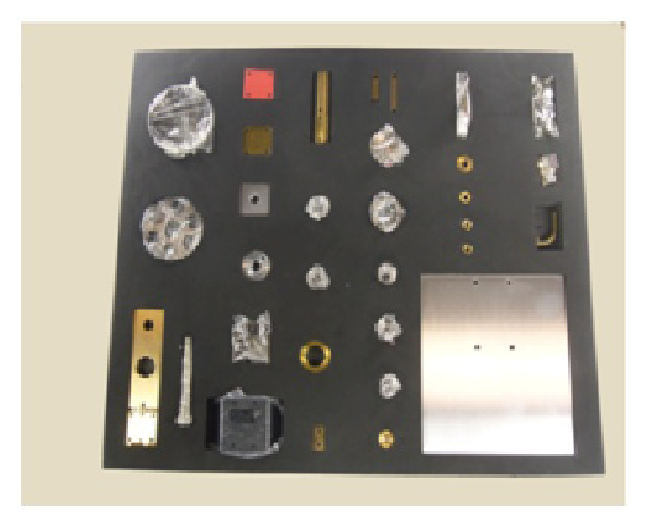
\includegraphics[width=6cm]{kit.eps}
\end{tabular}
\end{center}
\caption{Example kit (courtesy of http://littlemachineshop.com/).}
\label{fig:kit}
\end{figure}
Kitting is the process in which several different, but related items are placed into a container and supplied together as a single unit (kit) as shown in Figure~\ref{fig:kit}. Kitting is often performed prior to final assembly in industrial assembly of manufactured products so all of the necessary parts are gathered in one location. Manufacturers utilize kitting due to its ability to provide cost savings including saving manufacturing or assembly space, reducing assembly workers' walking and searching times, and increasing line flexibility and balance.


In batch kitting, the kit's component parts may be staged in containers positioned in the workstation or may arrive on a conveyor. Component parts may be fixtured, for example, placed in compartments on trays, or may be in random orientations, for example placed in a large bin. In addition to the kit's component parts, the workstation usually contains a storage area for empty kit boxes as well as completed kits.


Kitting has not yet been automated in many industries where automation may be feasible. Consequently, the cost of building kits is higher than it could be~\cite{Balakirsky.IROS.2012}. We are addressing this problem by building models of the knowledge that will be required to operate an automated kitting workstation in an agile manufacturing environment. For our automated kitting workstation, we assume that a robot performs a series of pick-and-place operations in order to construct the kit. These operations include:
\begin{enumerate}
\item Pick up empty kit and place on work table.
\item Pick up multiple component parts and place in kit.
\item Pick up completed kit and place in full kit storage area.
\end{enumerate}

Each of these actions may be a compound action that includes other actions such as end-of-arm tool changes, path planning, and obstacle avoidance. Finished kits are moved to the assembly floor where components are picked from the kit for use in the assembly procedure. The kits are normally designed to facilitate component picking in the correct sequence for assembly. Component orientation may be constrained by the kit design in order to ease the pick-to-assembly process. Empty kits are returned to the kit building area for reuse.


\subsection{Manufacturing Kitting Ontology Description}

\begin{table}[!h!t]
\caption{Kitting object ontology overview.}
\label{tab:kittingonto}
\centering
\resizebox{295pt}{!}{%
\begin{tabular}{l}
\toprule
\class{SolidObject} \textit{PrimaryLocation} \textit{SecondaryLocation}
\\\midrule
\hspace{5 mm}\class{BoxyObject} \textit{Length} \textit{Width} \textit{Heigh}
\\\midrule
\hspace{10 mm}\class{WorkTable} \textit{SolidObject}
\\\midrule
\hspace{5 mm}\class{EndEffector} \textit{Description} \textit{Weight} \textit{Id} \textit{LoadWeight}
\\\midrule
\hspace{10 mm}\class{GripperEffector} \textit{SolidObject}
\\\midrule
\hspace{10 mm}\class{VacuumEffector} \textit{CupDiameter} \textit{Length}
\\\midrule
\hspace{15 mm}\class{VacuumEffectorMultiCup} \textit{ArrayNumber} \textit{ArrayRadius}
\\\midrule
\hspace{15 mm}\class{VacuumEffectorSingleCup}
\\\midrule
\hspace{5 mm}\class{EndEffectorChangingStation} \textit{EndEffectorHolders}
\\\midrule
\hspace{5 mm}\class{EndEffectorHolder} \textit{EndEffector}
\\\midrule
\hspace{5 mm}\class{Kit} \textit{Tray} \textit{DesignRef} \textit{Parts} \textit{Finished?}
\\\midrule
\hspace{5 mm}\class{KittingWorkstation} \textit{WorkTable} \textit{Robot} \textit{ChangingStation} \textit{AngleUnit} \textit{LengthUnit} \textit{WeightUnit}
\\
\hspace{32 mm} \textit{KitDesigns} \textit{OtherObstacles} \textit{Skus}
\\\midrule
\hspace{5 mm}\class{KitTray} \textit{SkuRef} \textit{Serialnumber}
\\\midrule
\hspace{5 mm}\class{LargeBoxWithEmptyKitTrays} \textit{LargeContainer} \textit{Trays}
\\\midrule
\hspace{5 mm}\class{LargeBoxWithKits} \textit{LargeContainer} \textit{Kits} \textit{KitDesignRef} \textit{Capacity}
\\\midrule
\hspace{5 mm}\class{LargeContainer} \textit{SkuRef} \textit{SerialNumber}
\\\midrule
\hspace{5 mm}\class{Part} \textit{SkuRef} \textit{SerialNumber}
\\\midrule
\hspace{5 mm}\class{PartsBin} \textit{PartQuantity} \textit{PartSkuRef} \textit{SkuRef} \textit{SerialNumber}
\\\midrule
\hspace{5 mm}\class{PartsTray} \textit{SkuRef} \textit{SerialNumber}
\\\midrule
\hspace{5 mm}\class{PartsTrayWithParts} \textit{PartTray}
\\\midrule
\hspace{5 mm}\class{Robot} \textit{Description} \textit{MaximumLoadWeight} \textit{EndEffector} \textit{WorkVolume}
\\\midrule
\hspace{5 mm}
\\\midrule
\class{DataThing}
\\\midrule
\hspace{5 mm}\class{BoxVolume} \textit{MaximumPoint} \textit{MinimumPoint}
\\\midrule
\hspace{5 mm}\class{KitDesign} \textit{KitTraySkuRef} \textit{PartRefAndPoses}
\\\midrule
\hspace{5 mm}\class{PartRefAndPose} \textit{SkuRef} \textit{Point} \textit{XAxis} \textit{ZAxis}
\\\midrule
\hspace{5 mm}\class{PhysicalLocation} \textit{RefObject}
\\\midrule
\hspace{10 mm}\class{PoseLocation} \textit{Point} \textit{XAxis} \textit{ZAxis}
\\\midrule
\hspace{15 mm}\class{PoseLocationIn}
\\\midrule
\hspace{15 mm}\class{PoseLocationOn}
\\\midrule
\hspace{15 mm}\class{PoseOnlyLocation}
\\\midrule
\hspace{10 mm}\class{RelativeLocation} \textit{Description}
\\\midrule
\hspace{15 mm}\class{RelativeLocationIn}
\\\midrule
\hspace{15 mm}\class{RelativeLocationOn}
\\\midrule
\hspace{5 mm}\class{Point} \textit{X} \textit{Y} \textit{Z}
\\\midrule
\hspace{5 mm}\class{ShapeDesign} \textit{Description}
\\\midrule
\hspace{10 mm}\class{BoxyShape} \textit{Length} \textit{Width} \textit{Height} \textit{HasTop}
\\\midrule
\hspace{5 mm}\class{StockKeepingUnit} \textit{Description} \textit{Shape} \textit{Weight} \textit{EndEffectorRefs}
\\\midrule
\hspace{5 mm}\class{Vector} \textit{I} \textit{J} \textit{K}
\\\bottomrule
\end{tabular}
}
\end{table}

An industrial kitting ontology has been developed which will serve as the basis for the Industrial Robotics Ontology as part of the IEEE Robotics and Automation Society's (RAS) Ontologies for Robotics and Automation (ORA) Standard Working Group\footnote{http://lissi.fr/ora/doku.php}.The kitting workstation model was defined in OWL's functional-style syntax.

The model has two top-level classes, \textsf{SolidObject} and \class{DataThing}, from which all other classes are derived. \class{SolidObject} models solid objects, things made of matter. \class{DataThing} models data. Subclasses of \class{SolidObject} and \class{DataThing} are defined as shown in Table~\ref{tab:kittingonto}. The level of indentation indicates subclassing. For example, \class{WorkTable} is derived from \class{BoxyObject}, and \class{BoxyObject} is derived from \class{SolidObject}. Items in italics following classes are names of class attributes. Derived types inherit the attributes of the parent. Each attribute has a specific type not shown in the listing below. If an attribute type has derived types, any of the derived types may be used.

Each \class{SolidObject} has a native coordinate system conceptually fixed to the object. The native coordinate system of a \class{BoxyObject}, for example, has its origin at the middle of the bottom of the object, its Z axis perpendicular to the bottom, and the X axis parallel to the longer horizontal edges of the object.
\begin{table}[!t!h]
\caption{Preconditions and effects for the action \op{take-kittray}}
\label{tab:takekittray}
\begin{center}
\begin{tabular}{ll}
  \textit{preconditions} & \textit{effects} \\
  \hline
  \stvar{robot-empty}(\const{robot})&$\neg$\stvar{robot-empty}(\const{robot})\\\hline
  \stvar{lbwekt-not-empty}(\const{lbwekt})&\stvar{kittray-loc-robot}(\const{kittray},\const{robot})\\\hline
  \stvar{robot-with-endeffector}(\const{robot},\const{eeff})&\stvar{robot-holds-kittray}(\const{robot},\const{kittray})\\\hline
  \stvar{kittray-loc-lbwekt}(\const{kittray},\const{lbwekt})& $\neg$\stvar{kittray-loc-lbwekt}(\const{kittray},\const{lbwekt}) \\\hline

  \stvar{endeffector-loc-robot}(\const{eeff},\const{robot})&\\\hline
  \stvar{worktable-empty}(\const{worktable})& \\\hline
  \stvar{endeffector-type-kittray}(\const{eeff},\const{kittray})&\\\hline
\end{tabular}
\end{center}
\end{table}
In addition to representing objects, the ontology also represents activities. To represent activities in the manufacturing kitting ontology, both the actions and the pre- and post-conditions of those actions need to be represented. Preconditions and post-conditions (effects) are a combination of predicates. An example of action is \op{take-kittray} (take kit tray) which is defined as \op{take-kittray}(\const{robot},\const{kittray},\const{lbwekt},\const{eeff},\const{worktable}). In natural language, the \op{take-kittray} action involves a robot (\const{robot}) equipped with an end effector (\const{eeff}) picking up a kit tray (\const{kittray}) from within a large box with empty kit trays (\const{lbwekt}). This action is formally defined in the State Variable Representation~\cite{NAU.2004}. Table~\ref{tab:takekittray} shows the preconditions and effects (predicates) that are associated with this action.



Each of the predicates in Table~\ref{tab:takekittray} is described below:
\begin{enumerate}
\item \stvar{robot-empty}(\const{robot}) - TRUE iff robot (\const{robot}) is not holding anything
\item \stvar{lbwekt-not-empty}(\const{lbwekt}) - TRUE iff the large box with empty kit trays (\const{lbwekt}) is not empty
\item \stvar{robot-with-endeffector}(\const{robot},\const{eeff}) - TRUE iff robot (\const{robot}) is equipped with the end effector (\const{eeff})
\item \stvar{kittray-loc-lbwekt}(\const{kittray},\const{lbwekt}) - TRUE iff the kit tray (\const{kittray}) is in the large box with empty kit trays (\const{lbwekt})
\item \stvar{endeffector-loc-robot}(\const{eeff},\const{robot}) - TRUE iff the end effector (\const{eeff}) is being held by the robot (\const{robot})
\item \stvar{worktable-empty}(\const{worktable}) - TRUE iff there is nothing on the work table (\const{worktable})
\item \stvar{endeffector-type-kittray}(\const{eeff},\const{kittray}) - TRUE iff the end effector (\const{eeff}) is designed to handle the kit tray (\const{kittray})
\item $\neg$\stvar{robot-empty}(\const{robot}) - TRUE iff the robot (\const{robot}) is holding something
\item \stvar{kittray-loc-robot}(\const{kittray},\const{robot}) - TRUE iff the kit tray (\const{kittray}) is being held by the Robot (\const{robot})
\item \stvar{robot-holds-kittray}(\const{robot},\const{kittray}) - TRUE iff the Robot (\const{robot}) is holding the kit tray (\const{kittray})
\item $\neg$\stvar{kittray-loc-lbwekt}(\const{kittray},\const{lbwekt}) - TRUE iff the kit tray (\const{kittray}) is not in the large box with empty kit trays (\const{lbwekt})
\end{enumerate}

There are many other actions that can be performed during the kitting operation, including putting down a kit tray, picking up and putting down a part, attaching/removing an end effector, etc. Each of these actions has associated preconditions and effects

%%%%%%%%%%%%%%%%%%%%%%%%%%%%%%%%%%%%%%%%%%%%%%%%%%%%%%%%%%%%%%%%%%%%%%%%%%%%%%%%%%%%%
\section{Representing Manufacturing States}\label{S:section4}
%%%%%%%%%%%%%%%%%%%%%%%%%%%%%%%%%%%%%%%%%%%%%%%%%%%%%%%%%%%%%%%%%%%%%%%%%%%%%%%%%%%%%
When modeling the predicates in the preconditions and effects shown in the previous section, the first step is to precisely define the predicates in such a way as to determine if there were similar intermediate spatial relations that could be leveraged. We can start to formalize the previous definition of the predicates as depicted in the Revised Definition column in Table~\ref{tab:revised}.

\begin{center}
\begin{table}[!t!h]
\caption{Revised definitions of spatial relationships}
\label{tab:revised}
\centering
\scalebox{0.7}{
\begin{tabular}{lcc}
\toprule
\textbf{Predicate} & \textbf{Previous definition} & \textbf{Revised definition}\\\midrule
\stvar{lbwekt-not-empty}(\const{lbwekt}) &
\begin{minipage}[t]{0.22\columnwidth}%
TRUE iff the large box with empty kit trays (\const{lbwekt}) is not empty
\end{minipage} &
\begin{minipage}[t]{0.3\columnwidth}%
There is an object that is \textbf{Contained-In} the large box with empty kit trays (\const{lbwekt})
\end{minipage}
\\\midrule
\stvar{robot-with-endeffector}(\const{robot},\const{eeff}) &
\begin{minipage}[t]{0.22\columnwidth}%
TRUE iff robot (\const{robot}) is equipped with the end effector (\const{eeff})
\end{minipage} &
\begin{minipage}[t]{0.3\columnwidth}%
The end effector (\const{eeff}) is \textbf{In-Contact-With} the robot (\const{robot})
\end{minipage}
\\\midrule

\stvar{kittray-loc-lbwekt}(\const{kittray},\const{lbwekt}) &
\begin{minipage}[t]{0.22\columnwidth}%
TRUE iff the kit tray (\const{kittray}) is in the large box with empty kit trays (\const{lbwekt})
\end{minipage} &
\begin{minipage}[t]{0.3\columnwidth}%
The kit tray (\const{kittray}) is \textbf{Contained-In} the large box with empty kit trays (\const{lbwekt})
\end{minipage}
\\\midrule

\stvar{endeffector-loc-robot}(\const{eeff},\const{robot})&
\begin{minipage}[t]{0.22\columnwidth}%
TRUE iff the end effector (\const{eeff}) is being held by the robot (\const{robot})
\end{minipage} &
\begin{minipage}[t]{0.3\columnwidth}%
The end effector (\const{eeff}) is \textbf{In-Contact-With} the robot (\const{robot})
\end{minipage}
\\\midrule

\stvar{worktable-empty}(\const{worktable})&
\begin{minipage}[t]{0.22\columnwidth}%
TRUE iff there is nothing on the work table (\const{worktable})
\end{minipage} &
\begin{minipage}[t]{0.3\columnwidth}%
There is no object that is \textbf{On-Top-Of} and \textbf{In-Contact-With} the work table (\const{worktable})
\end{minipage}
\\\midrule

\stvar{endeffector-type-kittray}(\const{eeff},\const{kittray})&
\begin{minipage}[t]{0.22\columnwidth}%
TRUE iff the end effector (\const{eeff}) is designed to handle the kit tray (\const{kittray})
\end{minipage} &
\begin{minipage}[t]{0.3\columnwidth}%
The end effector (\const{eeff}) can handle the kit tray (\const{kittray})
\end{minipage}
\\\midrule

\stvar{kittray-loc-robot}(\const{kittray},\const{robot})&
\begin{minipage}[t]{0.22\columnwidth}%
TRUE iff the kit tray (\const{kittray}) is being held by the Robot (\const{robot})
\end{minipage} &
\begin{minipage}[t]{0.3\columnwidth}%
The kit tray (\const{kittray}) is \textbf{In-Contact-With} the robot (\const{robot}) and there is nothing \textbf{Under-And-In-Contact-With} the kit tray (\const{kittray})
\end{minipage}
\\\midrule

$\neg$\stvar{kittray-loc-lbwekt}(\const{kittray},\const{lbwekt})&
\begin{minipage}[t]{0.22\columnwidth}%
TRUE iff the kit tray (\const{kittray}) is not in the large box with empty kit trays (\const{lbwekt})
\end{minipage} &
\begin{minipage}[t]{0.3\columnwidth}%
The kit tray (\const{kittray}) is \textbf{Not-Contained-In} the large box with empty kit trays (\const{lbwekt})
\end{minipage}
\\\bottomrule
\end{tabular}
}
\end{table}
\end{center}

The predicates \stvar{robot-empty}, $\neg$\stvar{robot-empty}, and \stvar{robot-holds-kittray} depend on the type of effector that is being used to define the predicate. We will assume there are two types of end effectors: a vacuum end effector and a parallel gripper end effector. The vacuum end effector picks objects up by positioning itself on top of the object and uses air to create a vacuum to adhere to the object. The parallel gripper end effector picks objects up by squeezing them from both sides.  Because the vacuum end effector would not reasonably be used to pick up the kit tray, the \stvar{vacuum-holds-kittray}(\const{robot},\const{kittray}) state is not included below. In the case of the vacuum end effector, the relevant predicates would be:


\begin{itemize}
\item \stvar{vacuum-robot-empty}(\const{robot}) - there is no object \textbf{Under-And-In-Contact-With} the robot (\const{robot}) vacuum effector
\item $\neg$\stvar{vacuum-robot-empty}(\const{robot}) - there is an object \textbf{Under-And-In-Contact-With} the robot (\const{robot}) vacuum effector
\end{itemize}

In the case of the parallel gripper end effector, the predicates would be:
\begin{itemize}
\item \stvar{gripper-robot-empty}(\const{robot}) - there is no object \textbf{Partially-In-And-In-Contact-With} the robot (\const{robot}) gripper
\item $\neg$\stvar{gripper-robot-empty}(\const{robot}) - there is an object \textbf{Partially-In-And-In-Contact-With} the robot (\const{robot}) gripper
\item \stvar{gripper-holds-kittray}(\const{robot},\const{kittray}) - the kit tray (\const{kittray}) is \textbf{Partially-In-And-In-Contact-With} the robot (\const{robot}) gripper
\end{itemize}
\begin{figure}[h!t!]
\begin{center}
\begin{tabular}{c}
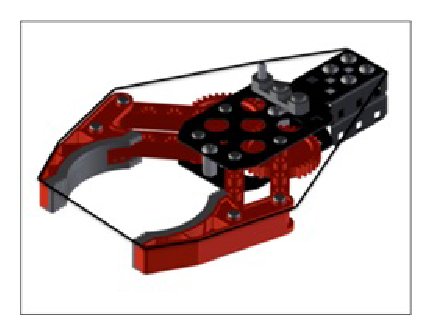
\includegraphics[width=6cm]{gripper.eps}
\end{tabular}
\end{center}
\caption{Convex hull around robot gripper.}
\label{fig:gripper}
\end{figure}
There is also one predicate that does not rely on spatial relations. The definition of \stvar{endeffector-type-kittray}(\const{eeff},\const{kittray}) states that a specific end effector must be able to be used on a kit tray. This information is included in the ontology class to describe the kit tray and therefore is out of scope of this document.

Also, in the manufacturing kitting domain, not all objects can be represented as convex regions, as is required by the RCC8 formalism. For example, the robot gripper in Figure~\ref{fig:gripper} is not convex and thus does not neatly fit into the RCC8 approach. To address this, we develop a convex hull along each relevant plane (as shown in Figure~\ref{fig:gripper}) around objects of this sort and use that convex hull to represent the region of the object in that plane.

Based on the manufacturing kitting ontology and the spatial relations, we can formally define the 11 manufacturing kitting predicates:

\begin{gather}
\label{eq:lbwekt-not-empty}
\stvar{lbwekt-not-empty}(\mathit{lbwekt}) \rightarrow \\
\class{SolidObject}(\textit{obj1}) \wedge \textbf{Contained-In}(\textit{obj1}, \mathit{lbwekt}) \notag
\end{gather}
\begin{gather}
\label{eq:robot-with-endeffector}
\stvar{robot-with-endeffector}(\mathit{robot},\mathit{eeff}) \rightarrow \\
\textbf{In-Contact-With}(\mathit{robot},\mathit{eeff}) \notag
\end{gather}
\begin{gather}
\label{eq:kittray-loc-lbwekt}
\stvar{kittray-loc-lbwekt}(\mathit{kittray},\mathit{lbwekt}) \rightarrow \\
\textbf{Contained-In}(\mathit{kittray},\mathit{lbwekt}) \notag
\end{gather}
\begin{gather}
\label{eq:worktable-empty}
\stvar{worktable-empty}(\mathit{worktable}) \rightarrow \\
\class{SolidObject}(\textit{obj1}) \wedge \neg\textbf{On-Top-Of}(\textit{obj1}, \mathit{worktable}) \wedge \notag\\
\neg \textbf{In-Contact-With}(\textit{obj1}, \mathit{worktable})\notag
\end{gather}
\begin{gather}
\label{eq:gripper-holds-kittray}
\stvar{gripper-holds-kittray}(\mathit{robot},\mathit{kittray}) \rightarrow \\
\class{GripperEffector}(\mathit{eeff}) \wedge \stvar{robot-with-endeffector}(\mathit{robot},\mathit{eeff}) \wedge \notag\\
\neg \textbf{Partially-In-And-In-Contact-With}(\mathit{kittray}, \mathit{eeff})\notag
\end{gather}
\begin{gather}
\label{eq:neg-kittray-loc-lbwekt}
\neg \stvar{kittray-loc-lbwekt}(\mathit{kittray},\mathit{lbwekt}) \rightarrow\\
\neg \textbf{Contained-In}(\mathit{kittray},\mathit{lbwekt}) \notag
\end{gather}
\begin{gather}
\label{eq:vacuum-robot-empty}
\stvar{vacuum-robot-empty}(\mathit{robot}) \rightarrow \\
\class{SolidObject}(\mathit{obj1}) \wedge \class{SolidObject}(\mathit{obj2}) \wedge \class{VacuumEffector}(\mathit{eeff}) \wedge\notag\\
\stvar{robot-with-endeffector}(\mathit{robot},\mathit{eeff}) \wedge \notag\\ \neg (\textbf{Under-And-In-Contact-With}(\mathit{obj1},\mathit{eeff}) \wedge \notag\\
\neg (\textbf{Under-And-With-Contact-With}(\mathit{obj2},\mathit{obj1}))\notag
\end{gather}
\begin{gather}
\label{eq:neg-vacuum-robot-empty}
\neg\stvar{vacuum-robot-empty}(\mathit{robot}) \rightarrow \\
\class{SolidObject}(\mathit{obj1}) \wedge \class{SolidObject}(\mathit{obj2}) \wedge \class{VacuumEffector}(\mathit{eeff}) \wedge\notag\\
\stvar{robot-with-endeffector}(\mathit{robot},\mathit{eeff}) \wedge \notag\\ \textbf{Under-And-In-Contact-With}(\mathit{obj1},\mathit{eeff}) \wedge \notag\\
\neg \textbf{Under-And-With-Contact-With}(\mathit{obj2},\mathit{obj1})\notag
\end{gather}
\begin{gather}
\label{eq:gripper-robot-empty}
\stvar{gripper-robot-empty}(\mathit{robot}) \rightarrow \\
\class{SolidObject}(\mathit{obj1}) \wedge \class{GripperEffector}(\mathit{eeff}) \wedge\notag\\
\stvar{robot-with-endeffector}(\mathit{robot},\mathit{eeff}) \notag
\end{gather}
\begin{gather}
\label{eq:neg-gripper-robot-empty}
\neg\stvar{gripper-robot-empty}(\mathit{robot}) \rightarrow \\
\class{SolidObject}(\mathit{obj1}) \wedge \class{GripperEffector}(\mathit{eeff}) \wedge\notag\\
\stvar{robot-with-endeffector}(\mathit{robot},\mathit{eeff}) \wedge\notag\\
\textbf{Partially-In-And-In-Contact-With}(\mathit{obj1},\mathit{eeff})\notag
\end{gather}
\begin{gather}
\label{eq:kittray-loc-robot}
\stvar{kittray-loc-robot}(\mathit{kittray},\mathit{robot}) \rightarrow \\
\stvar{gripper-holds-kittray}(\mathit{robot},\mathit{kittray}) \notag
\end{gather}


The formal definitions of these predicates will allow their existence to be recognized in a manufacturing environment, which in turn can be used by a state-based intention recognition system. The presence of predicates in certain predefined orders can help a robot recognize the intention of a human in the environment, which would allow the robot to better assist the human in performing upcoming activities.

%%%%%%%%%%%%%%%%%%%%%%%%%%%%%%%%%%%%%%%%%%%%%%%%%%%%%%%%%%%%%%%%%%%%%%%%%%%%%%%%%%%%%
\section{Experimentation and Results}\label{S:section5}
%%%%%%%%%%%%%%%%%%%%%%%%%%%%%%%%%%%%%%%%%%%%%%%%%%%%%%%%%%%%%%%%%%%%%%%%%%%%%%%%%%%%%

This section describes the experiments that were performed to validate the state recognition and representation approaches described in this paper. Though these states will be used as input to an intention recognition system, this part of the experiment only focused on the state recognition and representations aspects.

\subsection{Implementation Architecture and Description}

\begin{figure}[t!h!]
\begin{tabular}{c}
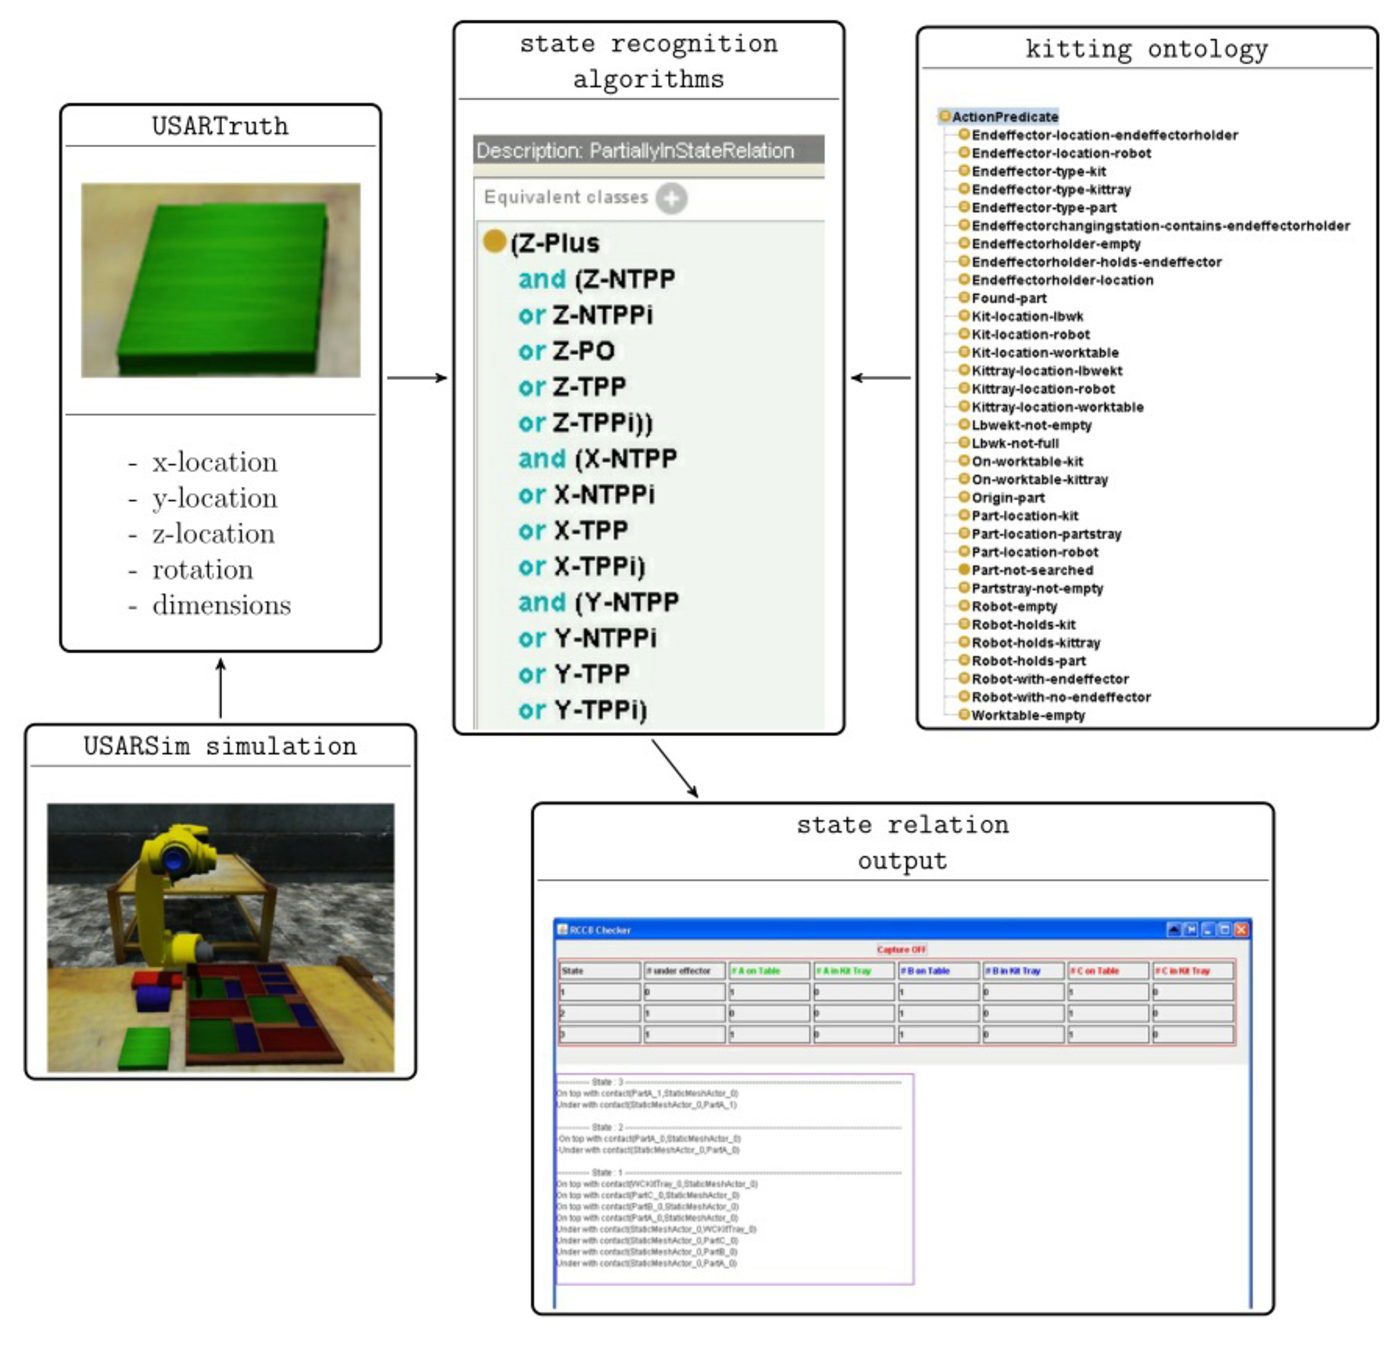
\includegraphics[width=13cm]{architecture.eps}
\end{tabular}
\caption{Implementation architecture.}
\label{fig:architecture}
\end{figure}
Figure~\ref{fig:architecture} shows the implementation architecture that was applied to the experiment. The evaluation was performed using the Unified System for Automation and Robot Simulation (\texttt{USARSim}) simulator~\cite{Carpin.ICRA.2007}. \texttt{USARSim} is a high-fidelity simulation of robots and environments based on the Unreal Tournament game engine. It is intended as a research tool and is the basis for the RoboCup rescue virtual robot competition~\cite{Kitano.ICAA.1997}. In this experiment, we used \texttt{USARSim} to simulate kitting operations. The \texttt{USARTruth} tool extracts ground truth data (the coordinates, the rotation, and the dimensions) of all objects in the simulated environment.

The ontology described earlier in this paper and the output from \texttt{USARTruth} are used as inputs to the \texttt{state recognition algorithms}. The \texttt{state recognition algorithms} parse the intermediate state relations and predicates in the ontology and extracts their equivalent classes. This is used to determine the logical formulas to analyze and link to the locations, rotations, and dimensions data retrieved from \texttt{USARTruth}. The algorithms first compute the truth-value of the RCC8 relationships in the ontology. The intermediate state relationships are then evaluated based on the truth-value of the RCC8 relationships, and finally the predicates are evaluated based on the truth-value of the intermediate state relationships. This process is run twice per second as new input is received from \texttt{USARTruth}. This frequency can be modified as needed.

\begin{figure}[t!h!]
\begin{center}
\begin{tabular}{c}
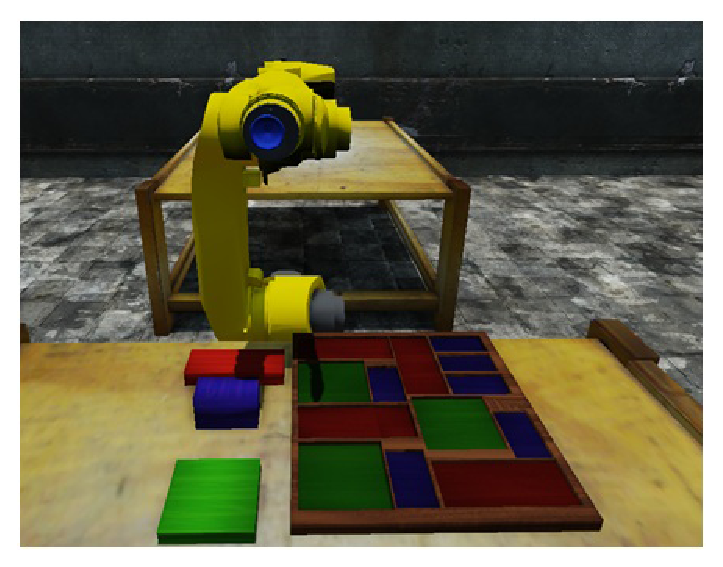
\includegraphics[width=7cm]{simulation.eps}
\end{tabular}
\end{center}
\caption{Scenario.}
\label{fig:scenario}
\end{figure}

A set of kitting scenarios was developed in \texttt{USARSim} to test the algorithms. All were industrial kitting scenarios, which involved different kit configurations, different parts, and different number of parts. One such scenario is shown in Figure~\ref{fig:scenario}. In this scenario, we use a robotic arm to represent a human arm performing actions. The kit that is being built contains three part A's (green), six part B's (blue) and four part C's (red). This is shown by the colors on the kit tray. As parts are picked up from the table, a new part of the same type is spawn. When the kit is finished, i.e., when the kit tray contains all the parts, the robot arm returns to its initial position.

\subsection{Output and Results}
Interestingly, in this industrial kitting scenario, there are relatively few state relationships that are relevant and of interest. They include:
\begin{itemize}
 \item Part A, B, or C is \sr{On-Top-Of} and \sr{In-Contact-With} the table
 \item Part A, B, or C is \sr{On-Top-Of} and \sr{In-Contact-With} the kit tray
 \item Part A, B, C is \sr{Under-And-In-Contact-With} the end effector
\end{itemize}

For the third bullet above, the spatial relation is \sr{Under-And-In-Contact-With} instead of \sr{Partially-In-And-In-Contact-With} because a vacuum effector is being used, which attaches to the part from the top and ``sucks it in". As such, the two are connected when the part is ``under and in contact with'' the end effector.

\begin{figure}[h!t!]
\begin{center}
\begin{tabular}{c}
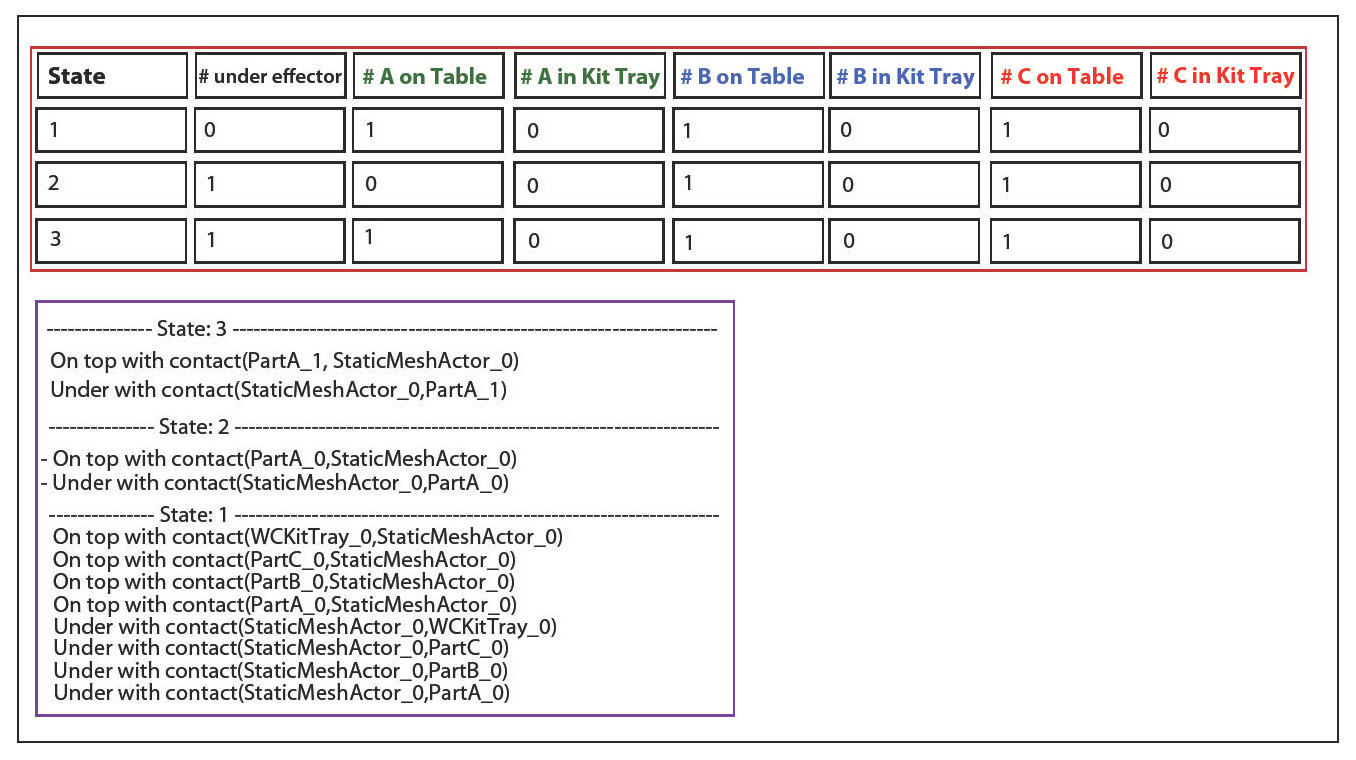
\includegraphics[width=13cm]{checker.eps}
\end{tabular}
\end{center}
\caption{State recognition algorithms output.}
\label{fig:staterecognition}
\end{figure}

Figure~\ref{fig:staterecognition} shows the output of the \texttt{state recognition algorithms} and consists of:
\begin{itemize}
 \item A table (top part in Figure~\ref{fig:staterecognition}) showing the number of parts held by the robot, the number and types of parts on the Table, and the number and types of Parts in the Kit Tray. Each of these is represented as columns in the table. Each row of the table represents a state.
 \item A textual description (bottom part in Figure~\ref{fig:staterecognition}) of all the predicates that are true in each state. State 1 displays all predicates that are true in that state. States 2,\ldots,$n$ show the predicates that have changed from the previous state. If a ``-" sign precedes the predicate name, the predicate is no longer true in the current state. The absence of a ``-" sign before the predicate name means that this predicate was not in the previous state and is now true in the current state.
\end{itemize}

In Figure~\ref{fig:staterecognition}, Parts A, B, and C are on the table and there are no parts in the kit tray for State 1. This is characterized by the three \texttt{On top with contact} relations (read as ``\textbf{On-Top-Of}" and ``\textbf{In-Contact-With}") between the parts and the table. A new state is established when a predicate-of-interest's truth-value changes. In State 2, the effector picked up Part A so Part A is under the effector and no longer on the table. In State 3, a new Part A appears on the table since the previous Part A has been picked up by the robot. This process will continue and new states will be defined until the kit assembly process is complete.



%%%%%%%%%%%%%%%%%%%%%%%%%%%%%%%%%%%%%%%%%%%%%%%%%%%%%%%%%%%%%%%%%%%%%%%%%%%%%%%%%%%%%
\section{Conclusion}\label{S:section6}
%%%%%%%%%%%%%%%%%%%%%%%%%%%%%%%%%%%%%%%%%%%%%%%%%%%%%%%%%%%%%%%%%%%%%%%%%%%%%%%%%%%%%
In this paper, we described a novel approach for representing state information for the purpose of intention recognition in cooperative human-robot environments. States were represented by a combination of spatial relationships in a Cartesian frame along with cardinal direction information. This approach was applied to a manufacturing kitting operation, where humans and robots are working together to develop kits.

The next step in this work is to apply the output of the state recognition algorithms to the ultimate goal of intention recognition. Each row in Figure  represents the predicates that are true at a given point of time (a state). The time ordering of these perceived predicates can be compared to predefined ordering of predicates that comprise an known intention. Future work will involve developing probabilistic algorithms to perform this comparison, thus allowing a robotic observer to infer what intention is most likely occurring by a human in the environment and then take actions to help advance that intention.

%%%%%%%%%%%%%%%%%%%%%%%%%%%%%%%%%%%%%%%%%%%%%%%%%%%%%%%%%%%%%%%%%%%%%
%\bibliographystyle{elsarticle-num}
\bibliographystyle{model6-num-names}
%\bibliographystyle{plain}
%\bibliographystyle{siam}
\bibliography{journal}
\end{document}

%%
%% End of file `elsarticle-template-num.tex'.
